\documentclass[12]{article}
\usepackage{amsmath}
\usepackage{amssymb}
\usepackage{graphicx}
\begin{document}
\title{Matix solving}
\maketitle
\section{Question}
A square, of each side 2, lies above the x-axis
and has one vertex at the origin. If one of the
sides passing through the origin makes an angle
30◦with the positive direction of the x-axis,
then find the sum of the x-coordinates of the
vertices of the square.
\section{solution}

\begin{figure}[h]
\centering
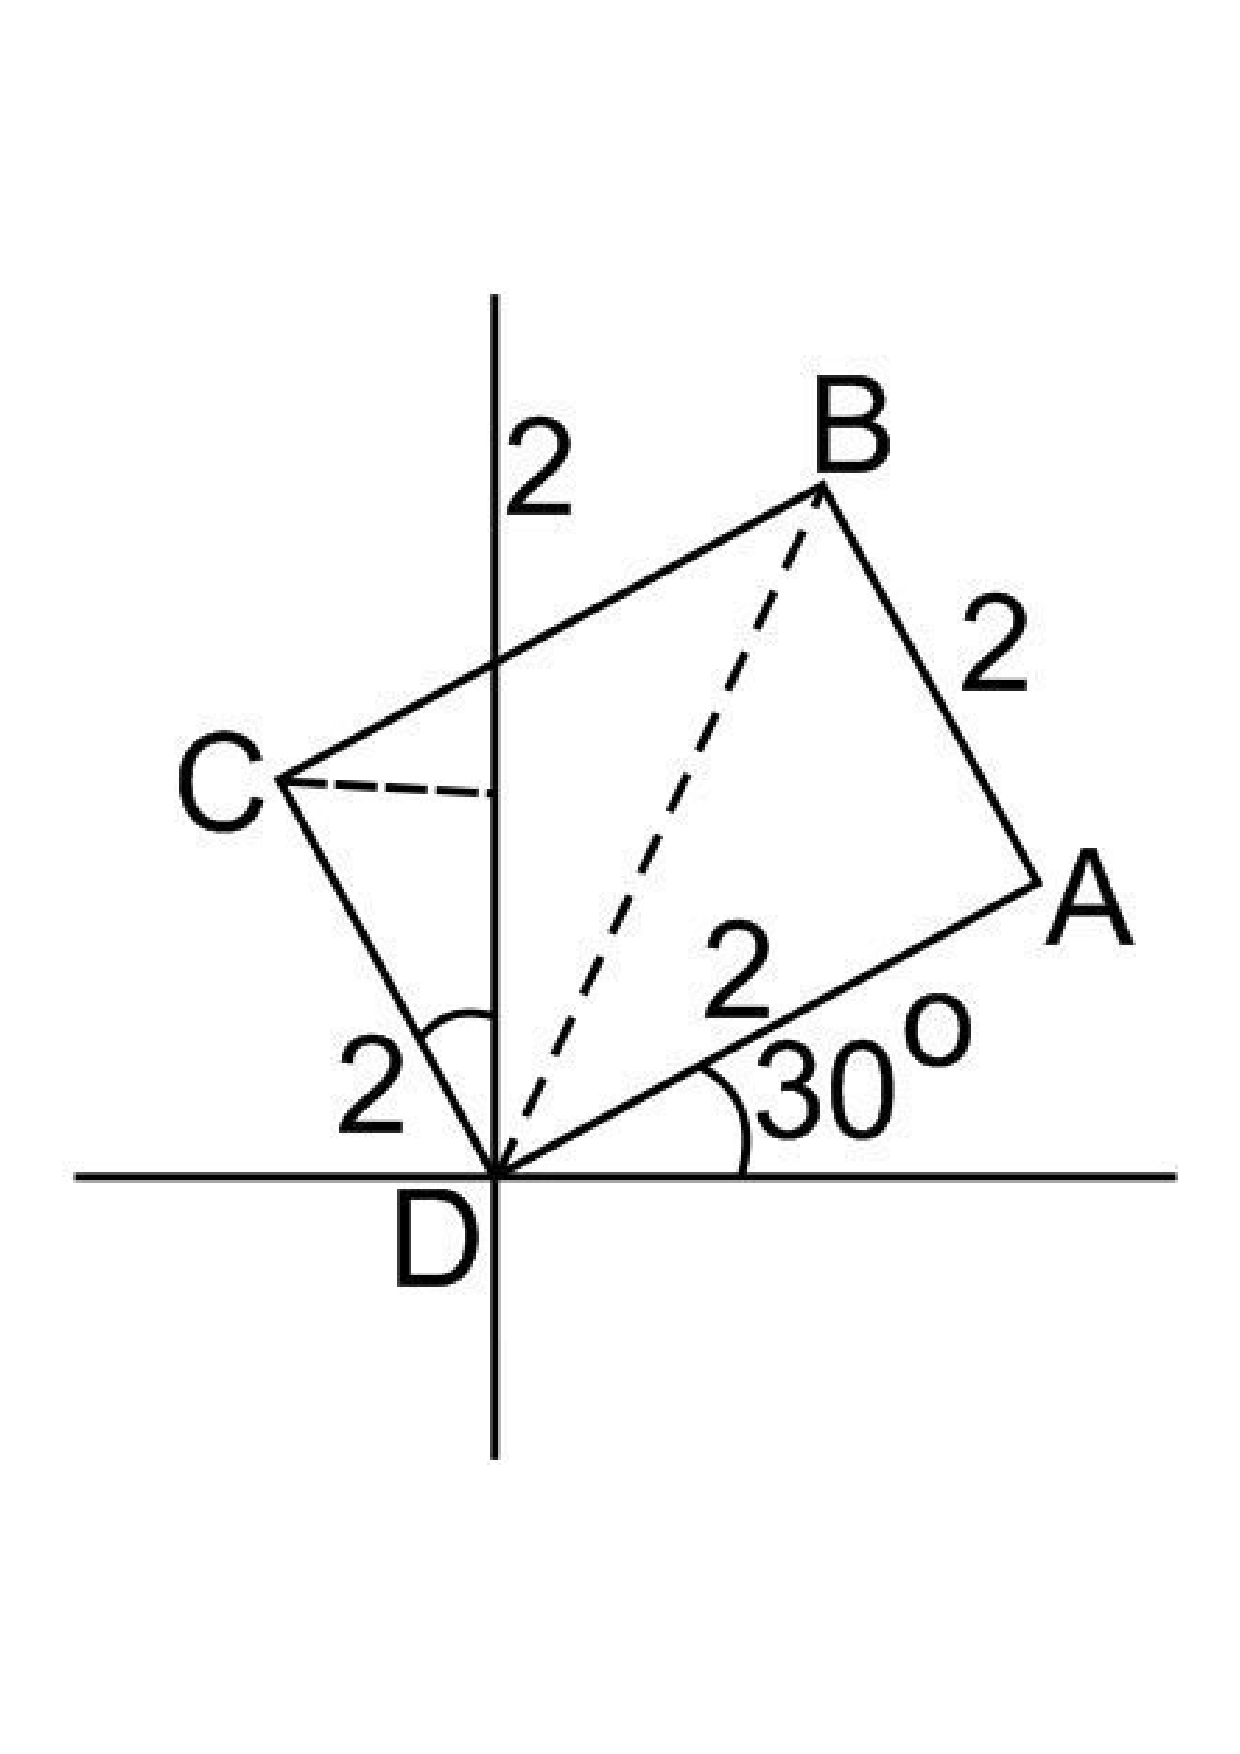
\includegraphics[scale=0.3]{square}
\end{figure}


Consider a line which has slope tan$\theta$ and passes through the point A(x1, y1).

Let P(x, y) be a point on the line which is at a distance r from the point A.

\begin{figure}[h]
\centering
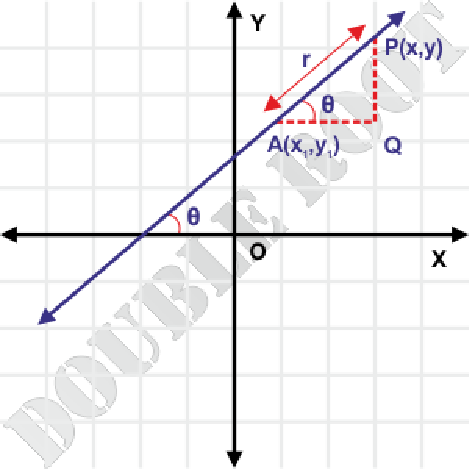
\includegraphics[scale=0.8]{parametriceq}
\end{figure}

We have, cos$\theta$ = AQ/AP = (x-x1)/r and sin$\theta$ = PQ/AP= (y-y1)/r

This gives the coordinates of P as (x1 + rcos$\theta$, y1 + rsin$\theta$).

And this is the parametric form of the equation of a straight line:  x = x1 + rcos$\theta$,  y = y1 + rsin$\theta$. 

This can also be written in a fancy way as x−x1/cos$\theta$=y−y1/sin$\theta$=r

Given length of side is 2 units and one of the vertex of the square is origin A(x1,y1)=(0,0)

Let other vertices be B,C,D

\begin{figure}[h]
\centering
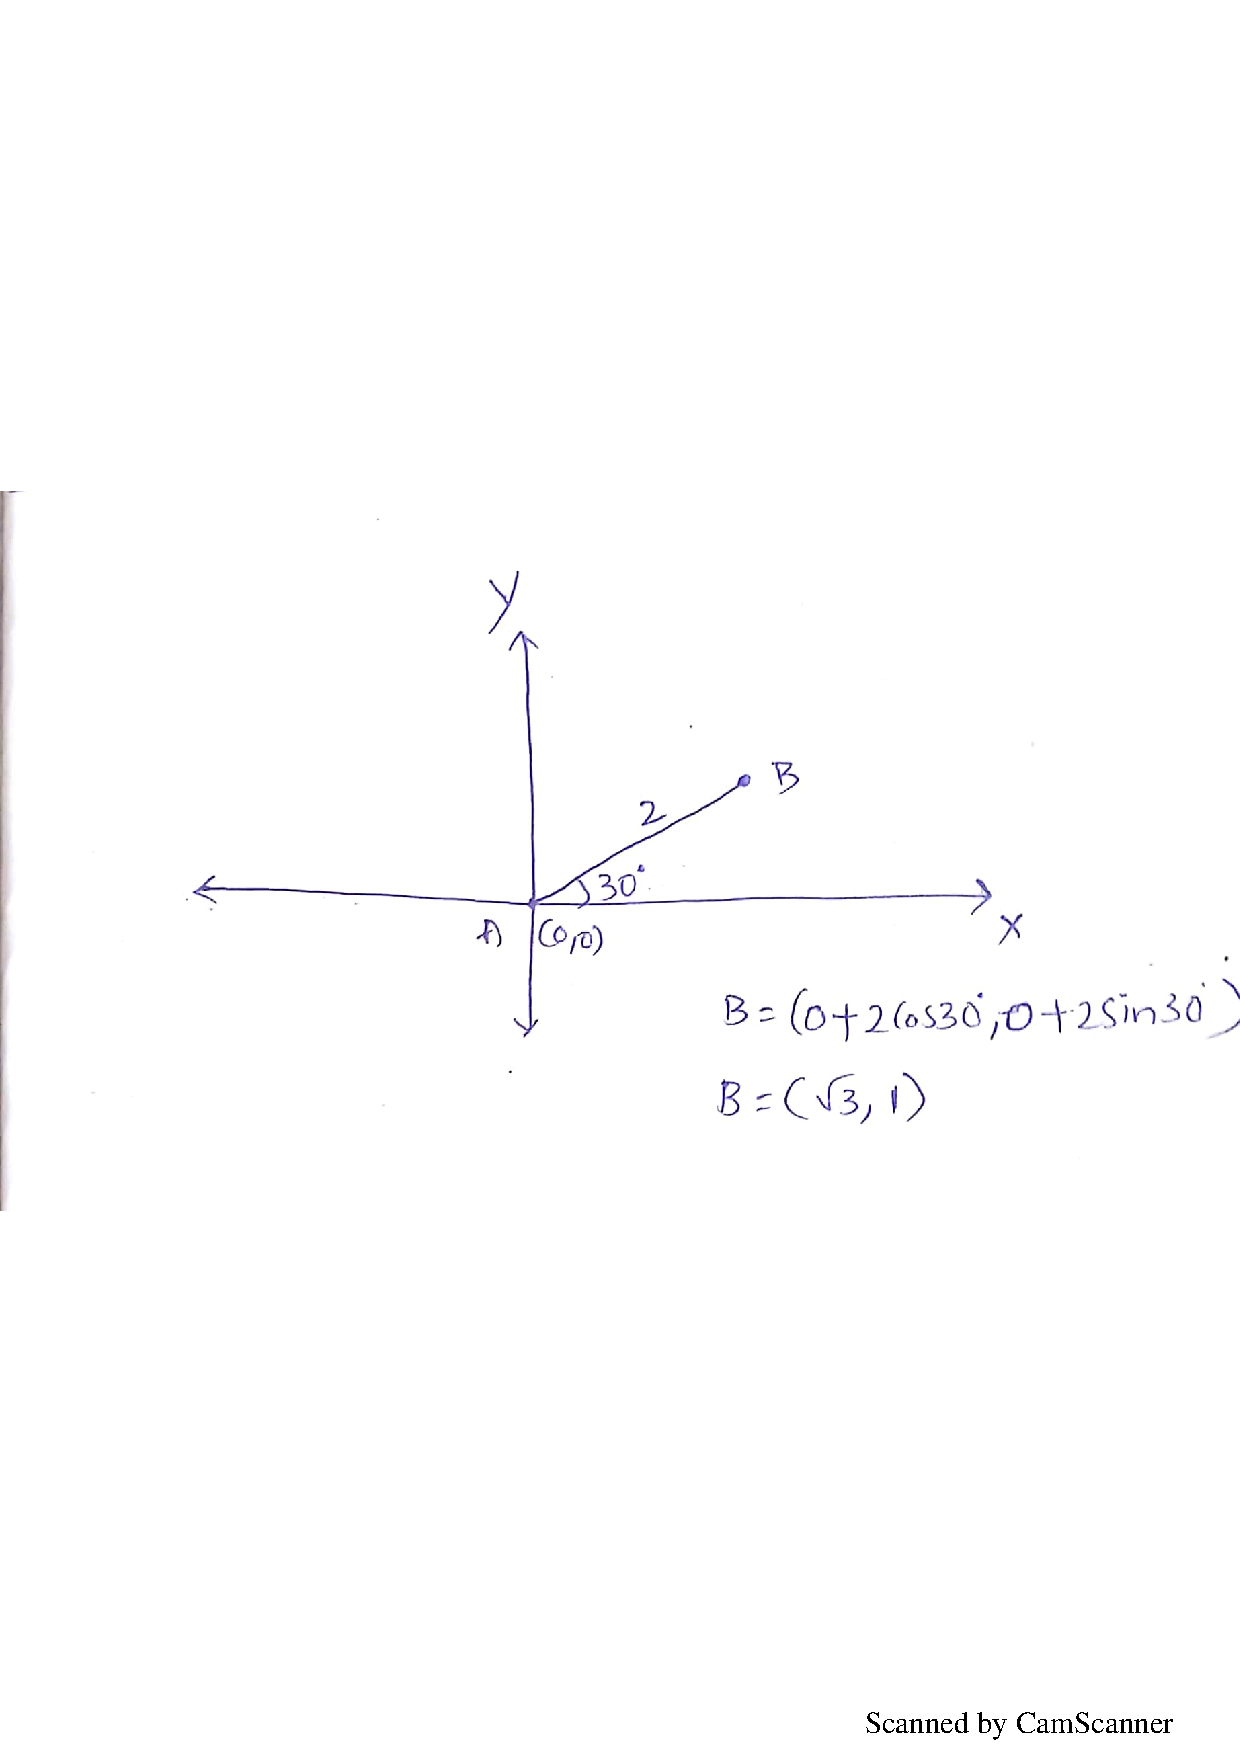
\includegraphics[scale=0.26]{pointB}
\end{figure}

Line AB makes an angle of 30degrees with the positive direction of x-axis in anticlockwise direction
then coordinates of the point which is 2 units away from origin and lie above x-axis (i.e Point B) can be written as

B(x2,y2)=(x1+2cos30$^\circ$ , x2+2sin30$^\circ$)

B(x2,y2)=(0+2cos30$^\circ$ , 0+2sin30$^\circ$)

B(x2,y2)=(\sqrt{3},1)

\begin{figure}[h]
\centering
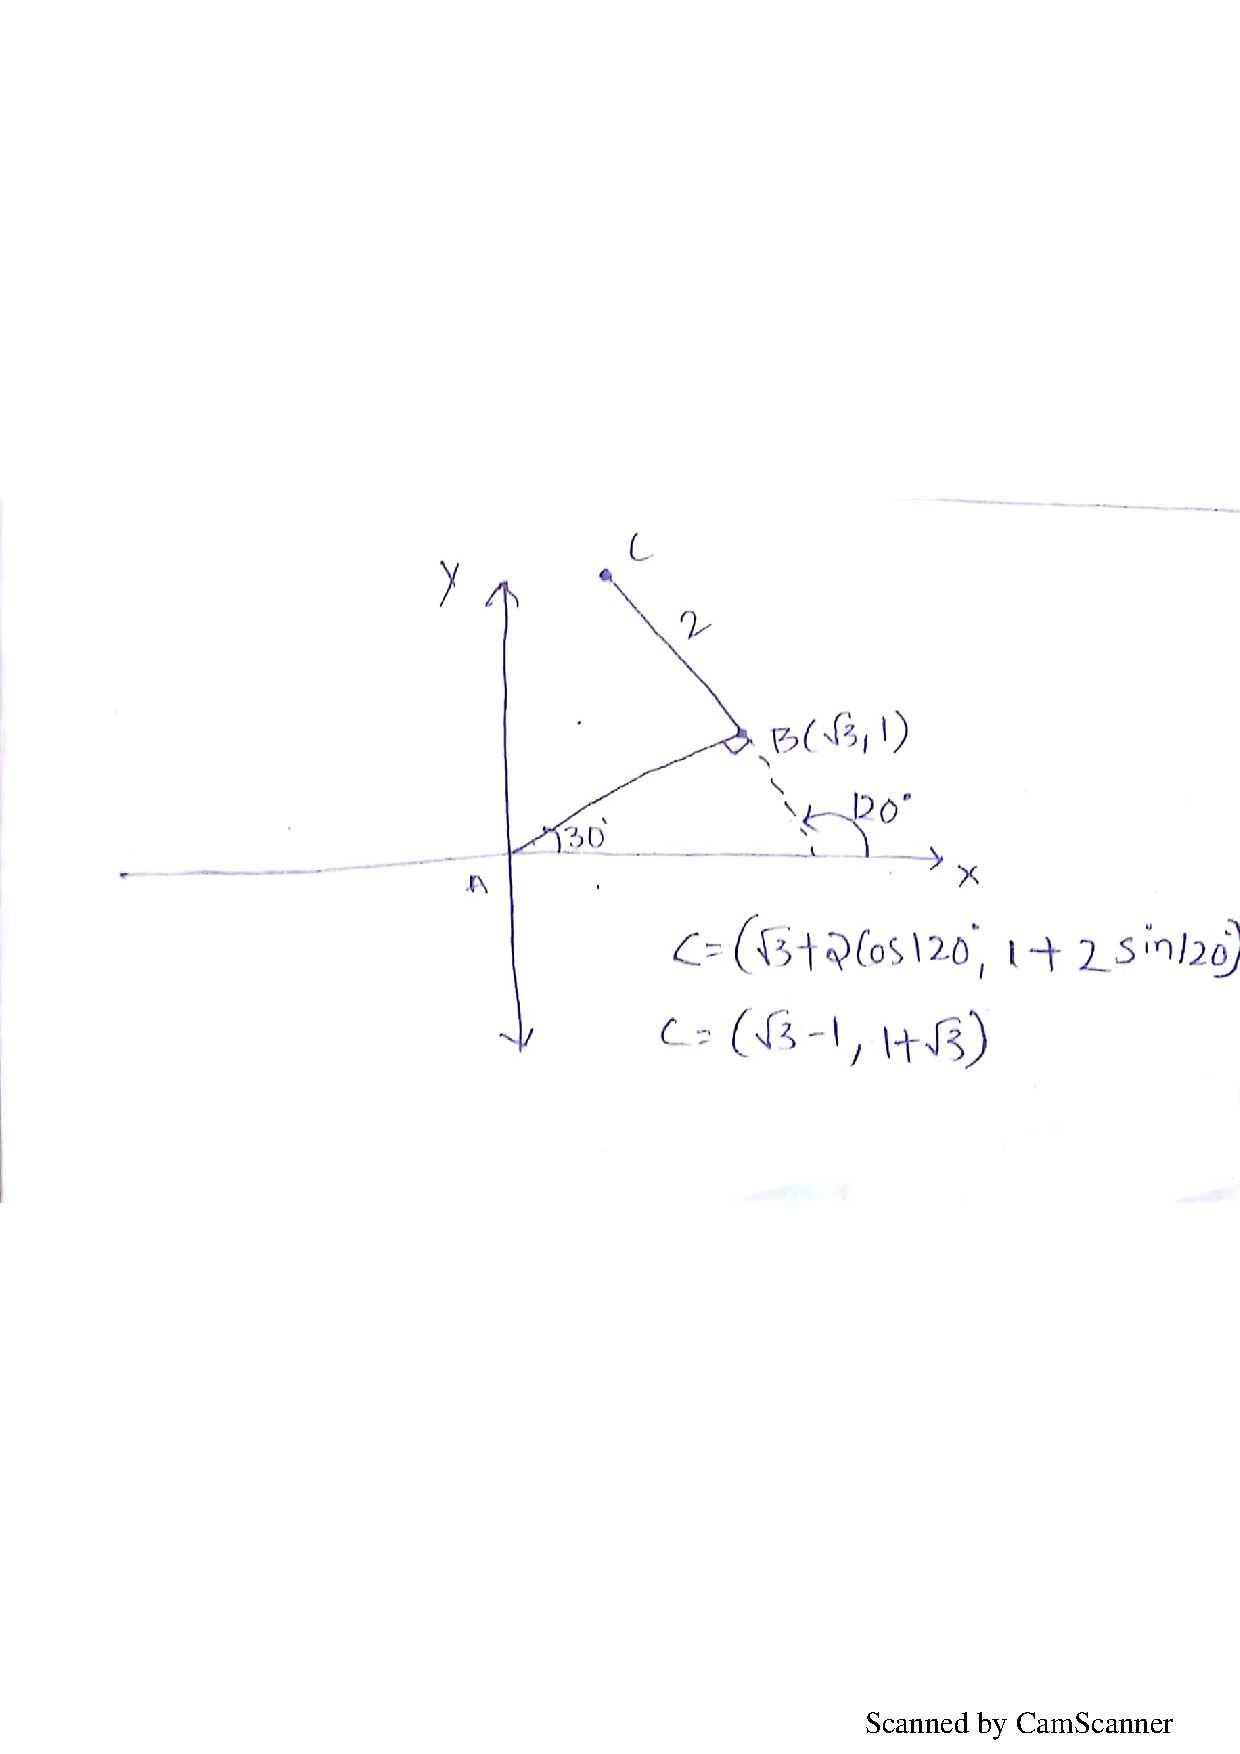
\includegraphics[scale=0.5]{pointC}
\end{figure}

Similarly line BC makes an angle of 120degrees(30+90) with the positive direction of x-axis in anticlockwise direction
then coordinates of the point which is 2 units away from B and lie above x-axis (i.e Point C) can be written as

C(x3,y3)=(x2+2cos(120)$^\circ$ , y2+2sin(120)$^\circ$)

C(x3,y3)=(\sqrt{3}+2cos(120)$^\circ$ , 1+2sin(120)$^\circ$)

C(x3,y3)=(\sqrt{3}-1,1+\sqrt{3})

\begin{figure}[h]
\centering
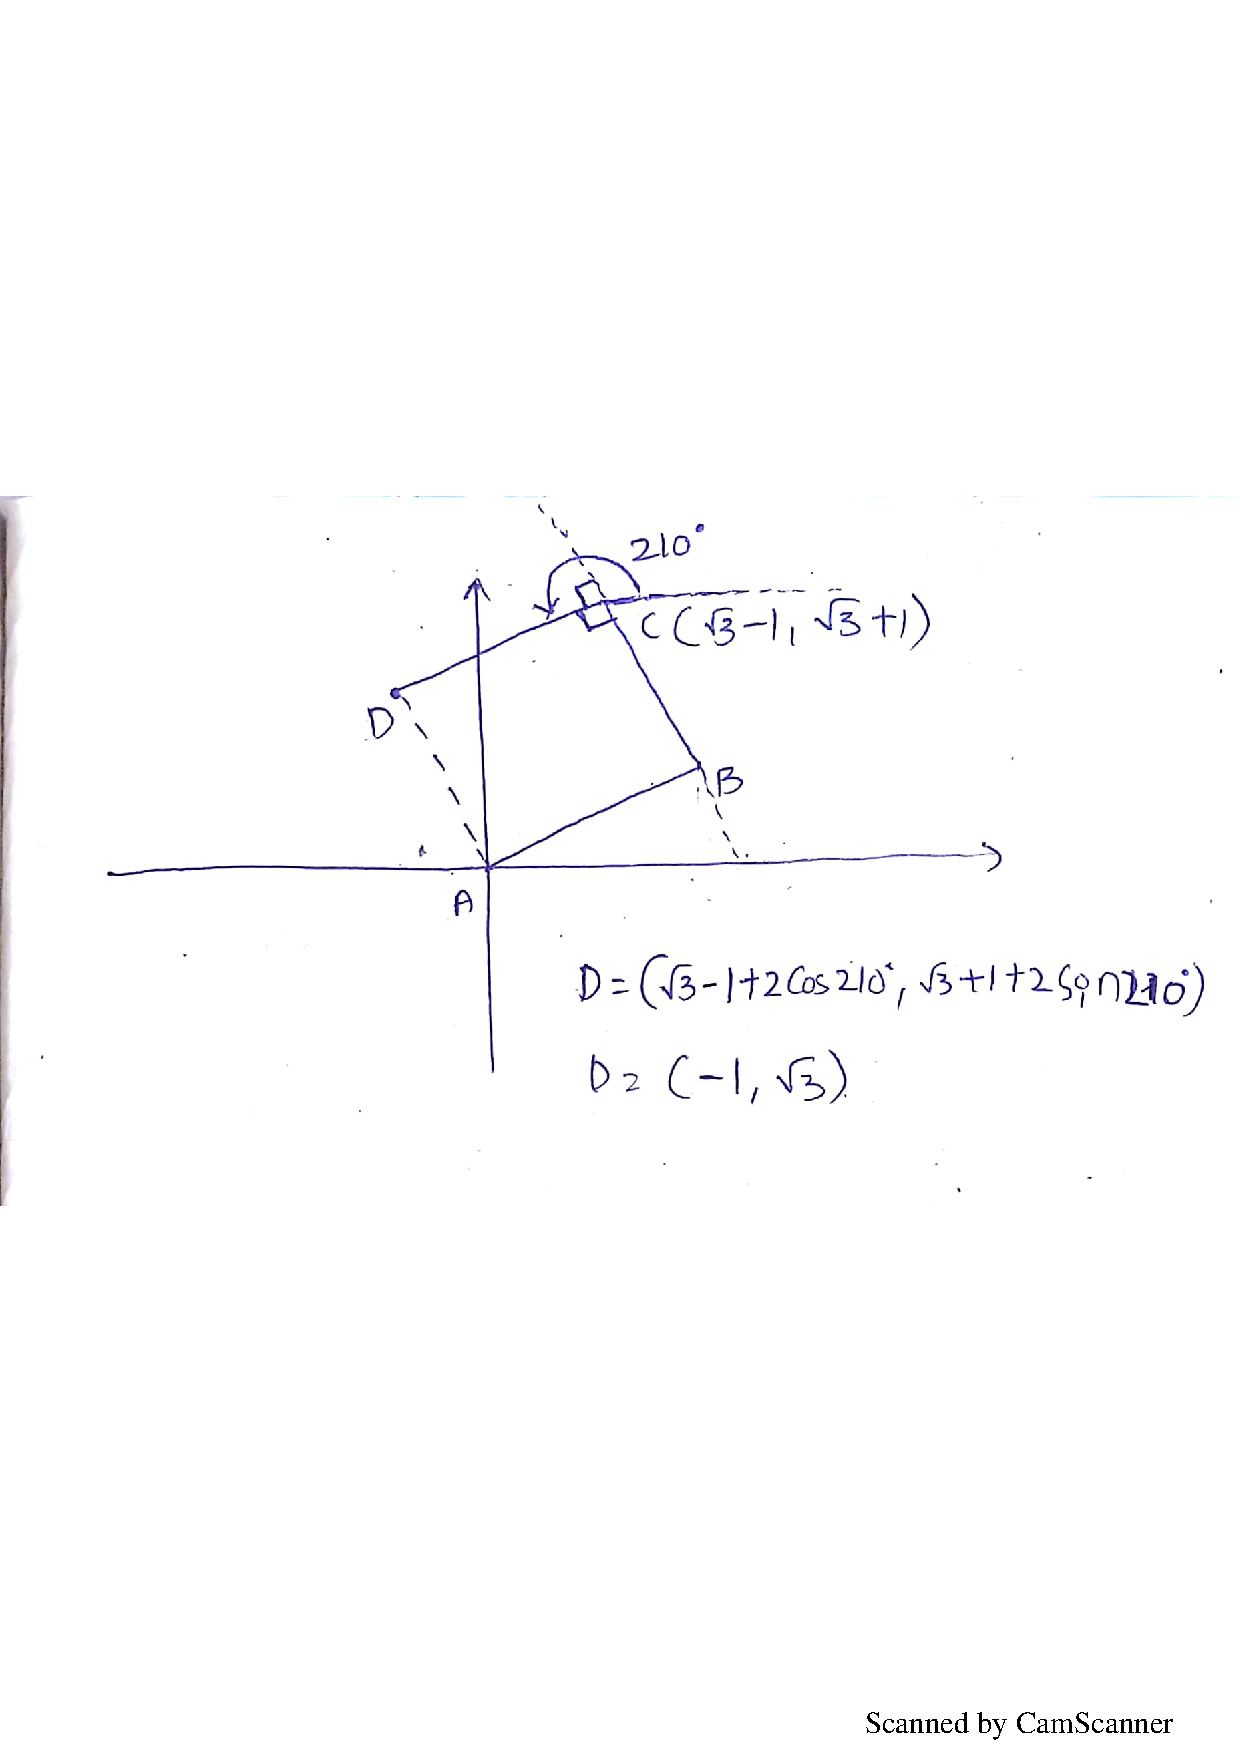
\includegraphics[scale=0.43]{pointD}
\end{figure}

Similarly line CD makes an angle of 210degrees(120+90) with the positive direction of x-axis in anticlockwise direction
then coordinates of the point(i.e Point D) which is 2 units away from C and also 2 units away from A (because it is a square) can be written as

D(x4,y4)=(x3+2cos(210)$^\circ$ , y3+2sin(210)$^\circ$)

D(x4,y4)=(\sqrt{3}-1+2cos(210)$^\circ$ ,\sqrt{3}+1+2sin(210)$^\circ$)

D(x4,y4)=(-1,\sqrt{3})

Let X be sum of x-cordinates

X=x1+x2+x3+x4

X=0+ \sqrt{3}+ (\sqrt{3}-1) + (-1)

X=1.464

\end{document} 